\begin{frame}[fragile]{strace}
  \begin{columns}
  \column{0.75\textwidth}
  \small
  System call tracer - \url{https://strace.io}
  \begin{itemize}
  \item Available on all GNU/Linux systems\\
        Can be built by your cross-compiling toolchain generator or by your build system.
  \item Allows to see what any of your processes is doing: accessing files, allocating memory...
        Often sufficient to find simple bugs.
  \item Usage:\\
    \code{strace <command>} (starting a new process)\\
    \code{strace -f <command>} ({\bf f}ollow child processes too)\\
    \code{strace -p <pid>} (tracing an existing process)\\
    \code{strace -c <command>} (time statistics per system call)
  \end{itemize}
  See \href{https://man7.org/linux/man-pages/man1/strace.1.html}{the strace manual} for details.
  \column{0.25\textwidth}
  \includegraphics[height=0.7\textheight]{common/strace-mascot.png}\\
  \tiny Image credits: \url{https://strace.io/}
  \end{columns}
\end{frame}

\begin{frame}[fragile]{strace example output}
  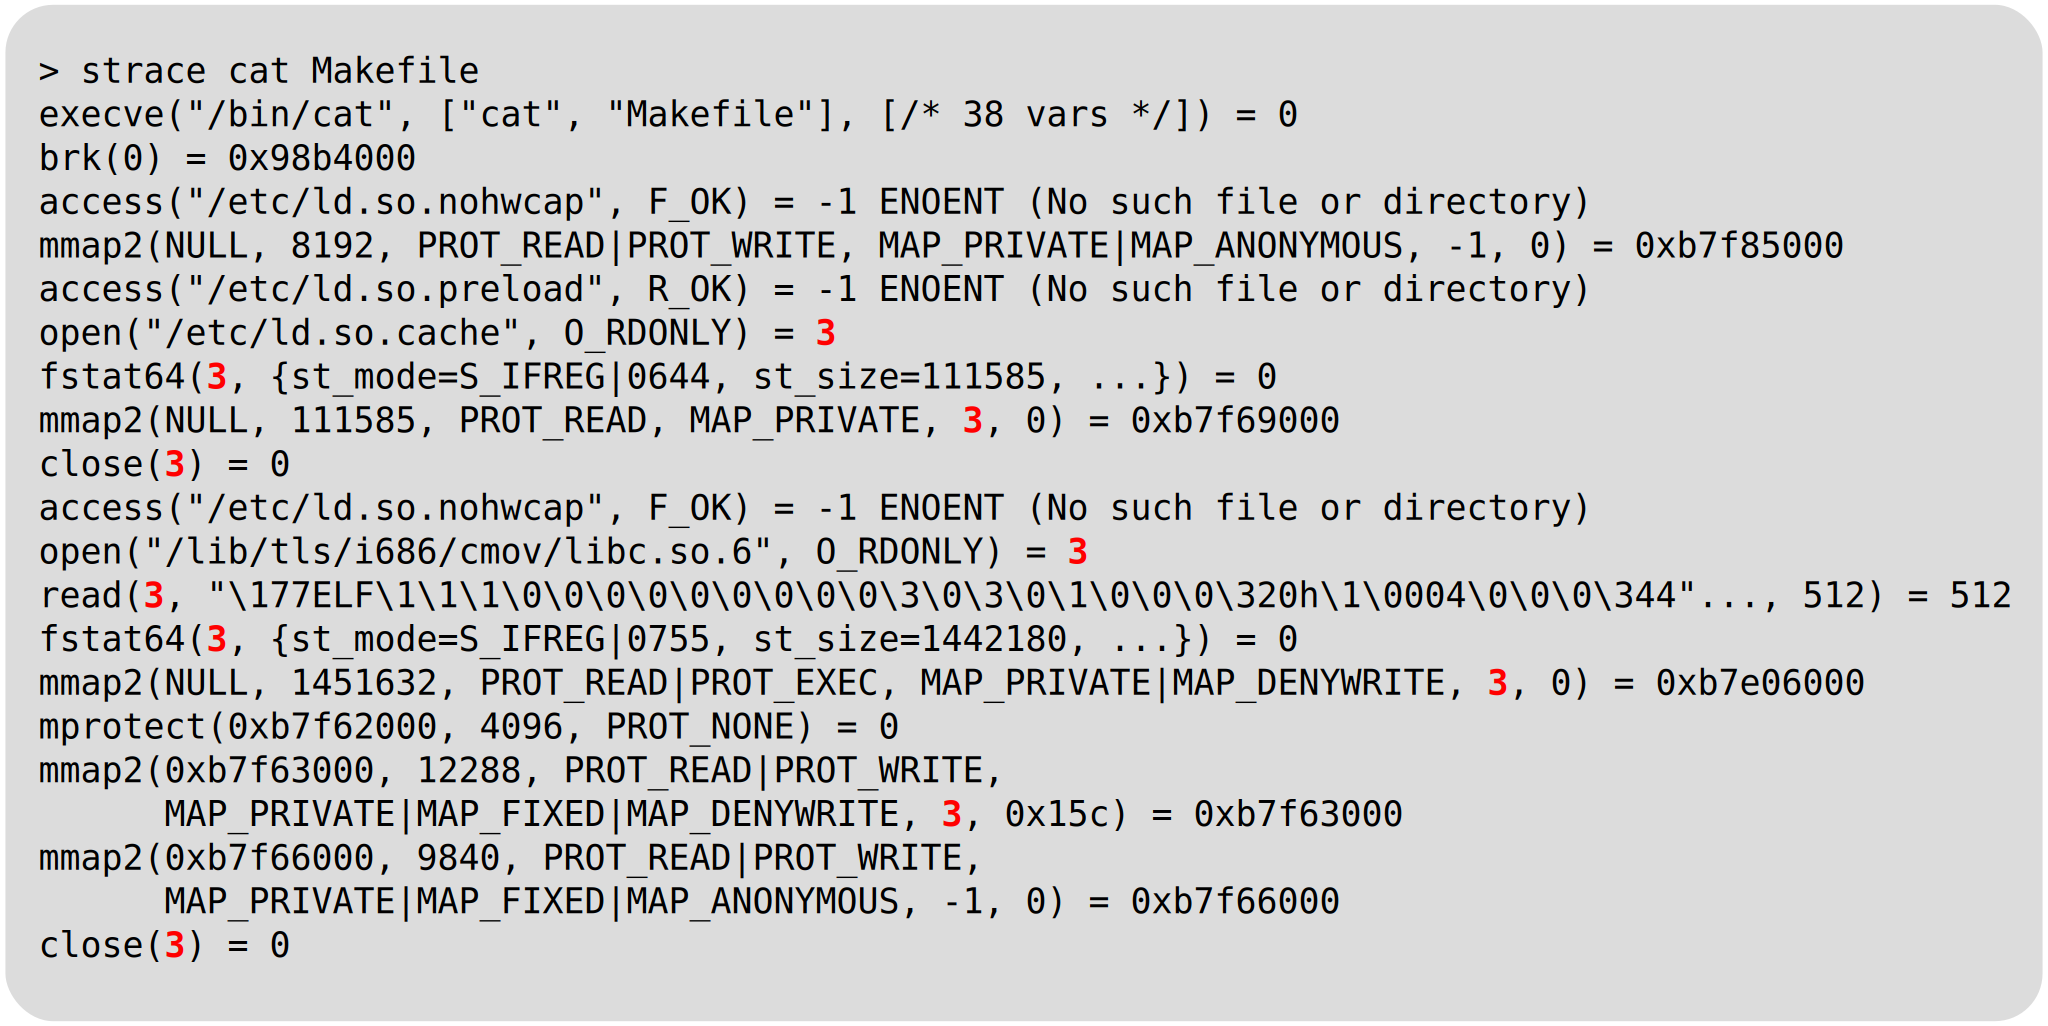
\includegraphics[height=0.75\textheight]{common/strace-output.pdf}\\
  Hint: follow the open file descriptors returned by \code{open()}.
  This tells you what files are handled by further system calls.
\end{frame}

\begin{frame}[fragile]
  \frametitle{strace -c example output}
  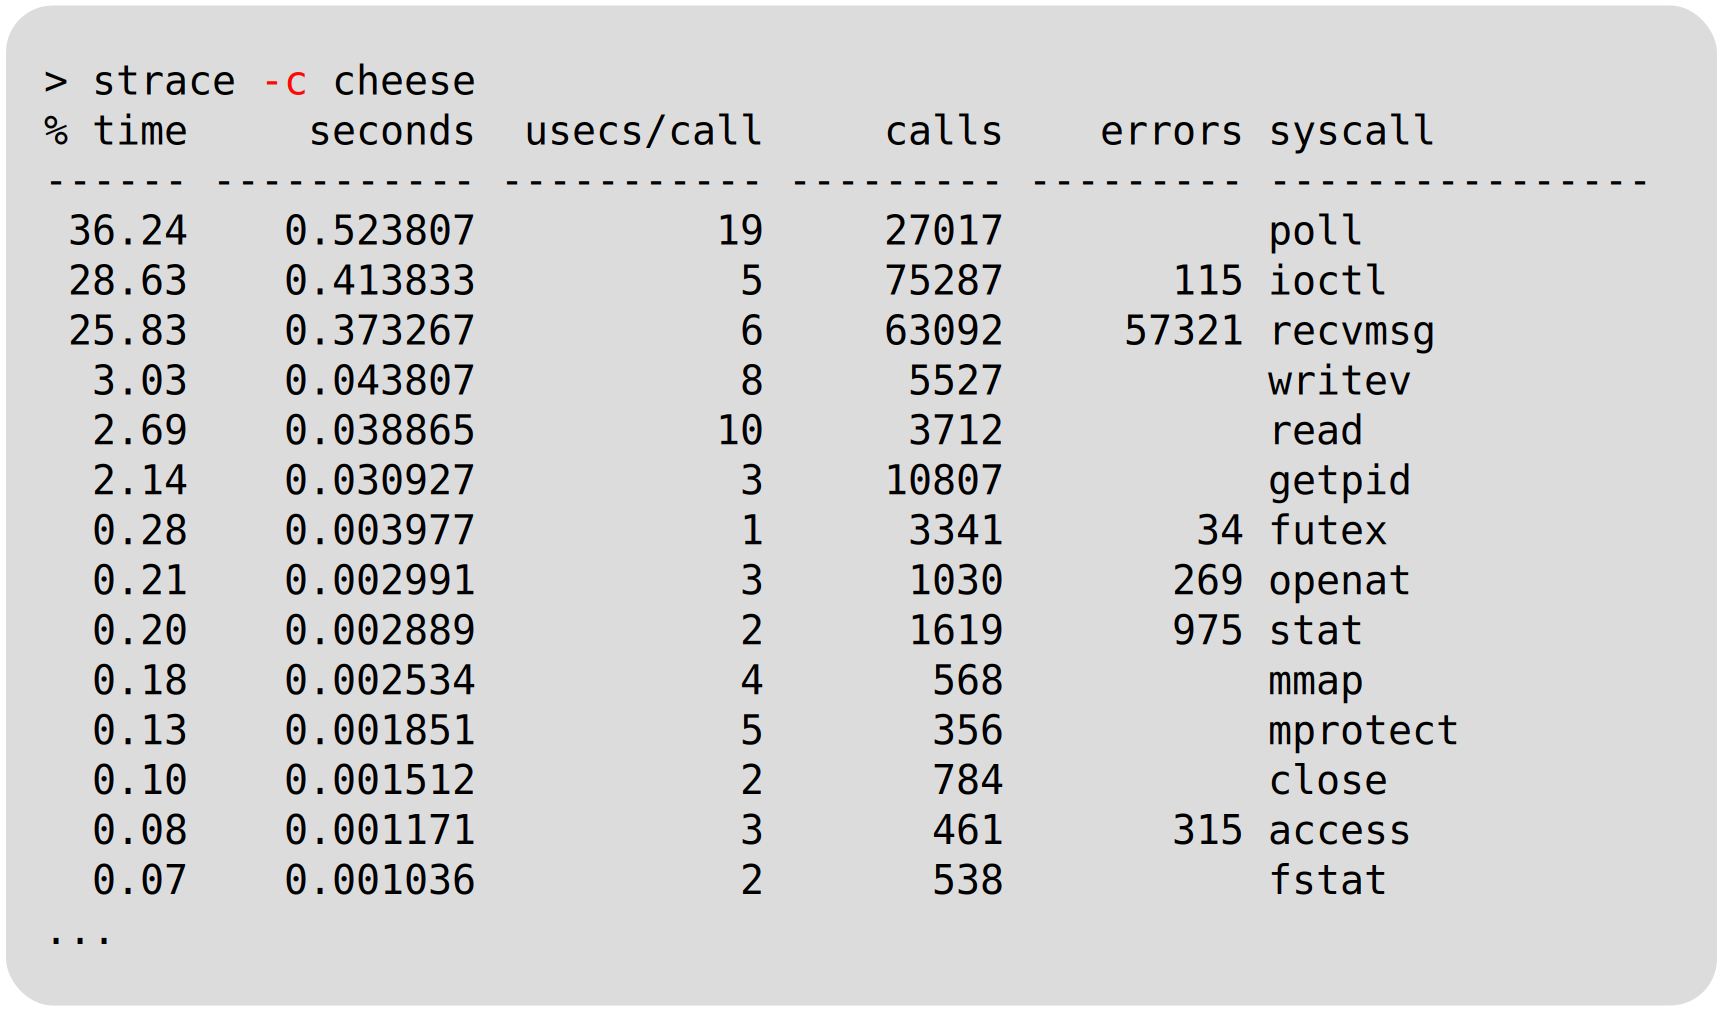
\includegraphics[height=0.8\textheight]{common/strace-c-output.pdf}
\end{frame}
